\newpage
%-------------------------------------------%
\section{Time Response Analysis}
%-------------------------------------------%
Higher order systems can be analysed by approximating them as 1\textsuperscript{st} or 2\textsuperscript{nd} order systems. 
%---------------EXAMPLE START---------------%
\begin{ex}{Mass-Spring-Damper system}
\begin{figure}[H] 
    \centering
    \begin{tikzpicture}[every node/.style={draw,outer sep=0pt,thick}]
    \tikzstyle{spring}=[thick,decorate,decoration={zigzag,pre length=0.3cm,post length=0.3cm,segment length=6}]
    \tikzstyle{damper}=[thick,decoration={markings,  
      mark connection node=dmp,
      mark=at position 0.5 with 
      {
        \node (dmp) [thick,inner sep=0pt,transform shape,rotate=-90,minimum width=15pt,minimum height=3pt,draw=none] {};
        \draw [thick] ($(dmp.north east)+(2pt,0)$) -- (dmp.south east) -- (dmp.south west) -- ($(dmp.north west)+(2pt,0)$);
        \draw [thick] ($(dmp.north)+(0,-5pt)$) -- ($(dmp.north)+(0,5pt)$) ; 
      }
    }, decorate]
    \tikzstyle{ground}=[fill,pattern=north east lines,draw=none,minimum width=0.75cm,minimum height=0.3cm]
    
    \node (M) [minimum width=1.5cm, minimum height=1.5cm] {$m$};
    \node (arrowstart) [name=arrowstart, above = 1cm of M.west,draw=none]{};
    \node (arrowend) [name=arrowend, above= 1cm of M.east,draw=none]{};
    
    \node (wall) [ground, rotate=-90, minimum width=1.5cm,yshift=-3cm] {};
    \draw (wall.north east) -- (wall.north west);
    
    % no need for ground, commented out
    % \node (gnd) [ground, rotate=0, minimum width=5cm,yshift=-0.9cm, xshift=-0.65cm] {};
    % \draw (wall.south east) -- (M.south east)--+(1.1cm,0);
    
    \draw [spring] (wall.160) -- ($(M.north west)!(wall.160)!(M.south west)$);
    \draw [damper] (wall.20) -- ($(M.north west)!(wall.20)!(M.south west)$);
    
    \draw [-latex,ultra thick] (M.east) ++ (0,0) -- +(1.1cm,0) node [above, draw=none]{$u(t)$} node [below=.15cm,draw=none]{Force};
    \draw [dashed] (M.east) ++ (0,0) -- +(0,1.5cm);
    \draw [-latex] (arrowstart) -- (arrowend) node[draw=none, above]{$y(t)$};
    
    \node[below=.3cm, draw=none] at (-2.1,-0.1){$c$};
    \node[above, draw=none] at (-2.1,0.5){$k$};
\end{tikzpicture}
\end{figure}
Impulse response: $g(t) = -e^{-\frac{1}{2}t}+ e^{-\frac{1}{3}t}$ with poles at $s=-\frac{1}{2}$, $s=-\frac{1}{3}$.\\\\
Recall that: The poles determine how quickly the system moves towards the steady state. Since $e^{-\frac{1}{2}t}$ decays faster than $e^{-\frac{1}{3}t}$, $s=-\frac{1}{3}$ is the dominant pole.\\\\
{\color{red}Dominant pole} lies closer to the imaginary axis in $s$-plane.
\begin{figure}[H] 
    \centering 
    \begin{tikzpicture}[>=latex]
    \begin{axis}[
      axis x line=center,
      axis y line=center,
      xtick = {-1/3, -1/2},
      xticklabels={$-\frac{1}{3}$, $-\frac{1}{2}$},
      yticklabels={,,},
      xlabel={$Re$},
      ylabel={$Im$},
      xlabel style={below right},
      ylabel style={above left},
      xmin=-0.6,
      xmax=0.2,
      ymin=-0.2,
      ymax=0.2,
      x=5cm, y=8cm/2]
    \addplot[
        scatter/classes={a={blue}, b={red}},
        scatter, mark=*, only marks, 
        scatter src=explicit symbolic 
    ] table [meta=class] {
        x y class
        -0.5 0 a 
        -0.333 0 b 
    };
    \end{axis}
\end{tikzpicture}
\end{figure}
\end{ex}
%----------------EXAMPLE END----------------%
%---------------EXAMPLE START---------------%
\begin{ex}{}
    Obtain the dominant pole approximation of $\displaystyle G(s) = \frac{10}{(s+10)(s^{2}+2s+2)}$.\\\\
    Poles $s=-10$ and $s = -1\pm j$, their locations are shown in the $s$-plane below. Since $s = -1 \pm j$ lie closer to the imaginary axis, these are {\color{red}Dominant poles} of the system.
    \begin{figure}[H] 
        \centering 
        \begin{tikzpicture}[>=latex]
    \begin{axis}[
      axis x line=center,
      axis y line=center,
      xtick = {-3, -0.5},
      xticklabels={10, $-1\pm j$},
      yticklabels={},
      xlabel={$Re$},
      ylabel={$Im$},
      xlabel style={below right},
      ylabel style={above left},
      xmin=-3.2,
      xmax=0.2,
      ymin=-1.2,
      ymax=1.2,
      x=1cm, 
      y=2cm/2]
    \addplot[
        scatter/classes={a={blue}, b={red}},
        scatter, mark=*, only marks, 
        scatter src=explicit symbolic 
    ] table [meta=class] {
        x y class
        -0.5 0.6 b 
        -0.5 -0.6 b 
        -3 0 a
    };
    \end{axis}
\end{tikzpicture}
    \end{figure}
    We can approximate the system by 
    \begin{itemize}
    \item keeping only the dominant poles
    \item ensuring the equal steady state for unit step response
    \end{itemize}
    For the case above, since $s = -1\pm j$ are the dominant poles:
    \[ G(s) = \frac{10}{(s+10)(s^{2}+2s+2)} \quad \to \quad \hat{G}(s) =\frac{K}{s^{2}+2s+2}\]
    To determine the value of $K$:
    \[\begin{cases}
    \displaystyle
    y(\infty) = \lim_{s\to 0}sY(s) = \lim_{s\to0}sG(s)\frac{1}{s} = \frac{1}{2} \quad \\
    \displaystyle
    \hat{y}(\infty) = \lim_{s\to 0}s\hat{Y}(s) = \lim_{s\to0}s\hat{G}(s)\frac{1}{s} = \frac{K}{2}\\
    \end{cases}\]
    $\therefore$ \quad $K = 1$.
\end{ex}
%----------------EXAMPLE END----------------%

%-------------------------------------------%
\subsection{Good and Bad Approximations}
%-------------------------------------------%
\begin{itemize}
    \item If the dominant poles are very different from the other poles, this will lead to a good approximation;
        \begin{ex}{}
            The system $\displaystyle G(s)=\frac{10}{(s+10)(s^{2}+2s+2)}$ has poles at $s = -10$, $s = -1 \pm j$. \\\\Since poles are not close each other, the 2\textsuperscript{nd} order approximation is almost equivalent to the original system.
            \begin{figure}[H] \centering 
                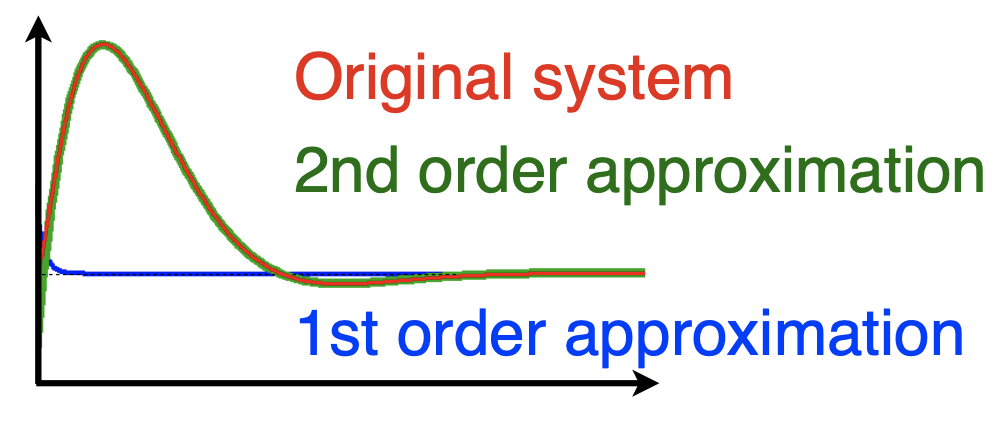
\includegraphics[width=.4\textwidth]{images/good_approx.png}
                \caption{A good approximation, $G(s)=\frac{10}{(s+10)(s^{2}+2s+2)}$}
            \end{figure}
        \end{ex}
    
    \item If the dominant pole is close to the other poles, the approximation will be imprecise.
    %---------------EXAMPLE START---------------%
        \begin{ex}{}
            The system $\displaystyle G(s)=\frac{1}{(s+51)(s^{2}+100s+9000)}$ has poles at $s = -51$, $s = -50 \pm 81j$.\\\\ In this case, poles are close to each other, which leads to the bad approximation.
            \begin{figure}[H] 
                \centering 
                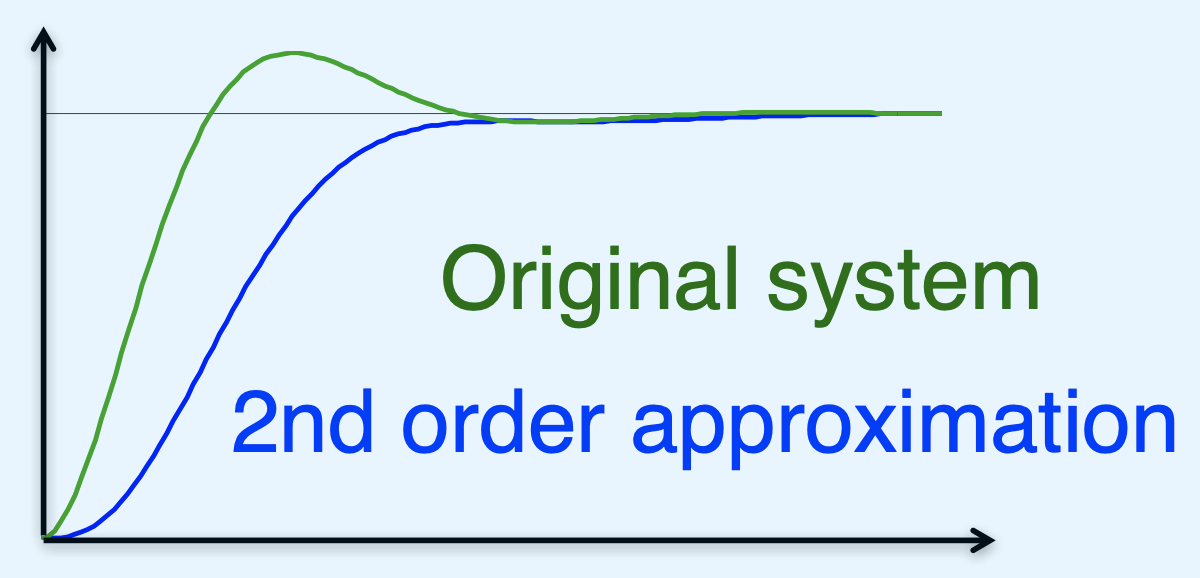
\includegraphics[width=.4\textwidth]{images/bad_approx.png}
                \caption{A bad approximation, $G(s)=\frac{1}{(s+51)(s^{2}+100s+9000)}$}
            \end{figure}
        \end{ex}
    %----------------EXAMPLE END----------------%
\end{itemize}
%-------------------------------------------%
\subsection{Time Response Analysis for 1\textsuperscript{st} Order Systems}
%-------------------------------------------%
\[
T\frac{\mathrm{d}y(t)}{\mathrm{d}t}+y(t)=Ku(t) 
\quad {\color{gray}\xleftrightarrow[\mathcal{L}^{-1}]{\mathcal{L}}} \quad  
(Ts+1)Y(s)=KU(s)
\]
\begin{itemize}
    \item The transfer function for a 1\textsuperscript{st} order system is $G(s)=\frac{K}{Ts+1}$ with poles at $s=-\frac{1}{T}$,  $T$ is known as the \textbf{time constant}. 
    \item Time constant determines how fast the system moves towards the steady state.
\end{itemize}

%-------------------------------------------%
\subsubsection{Impulse Response of 1\textsuperscript{st} Order Systems}
%-------------------------------------------%
\[
U(s)=1 
\quad {\color{gray}\longrightarrow} \quad 
\boxed{G(s)=\frac{K}{Ts+1}}
\quad {\color{gray}\longrightarrow} \quad 
Y(s)= \frac{K}{Ts+1} 
\quad {\color{gray}\xrightarrow[]{\mathcal{L}^{-1}}} \quad 
y(t) = \frac{K}{T}e^{-\frac{1}{T}t}
\]

\begin{figure}[H] 
    \centering 
    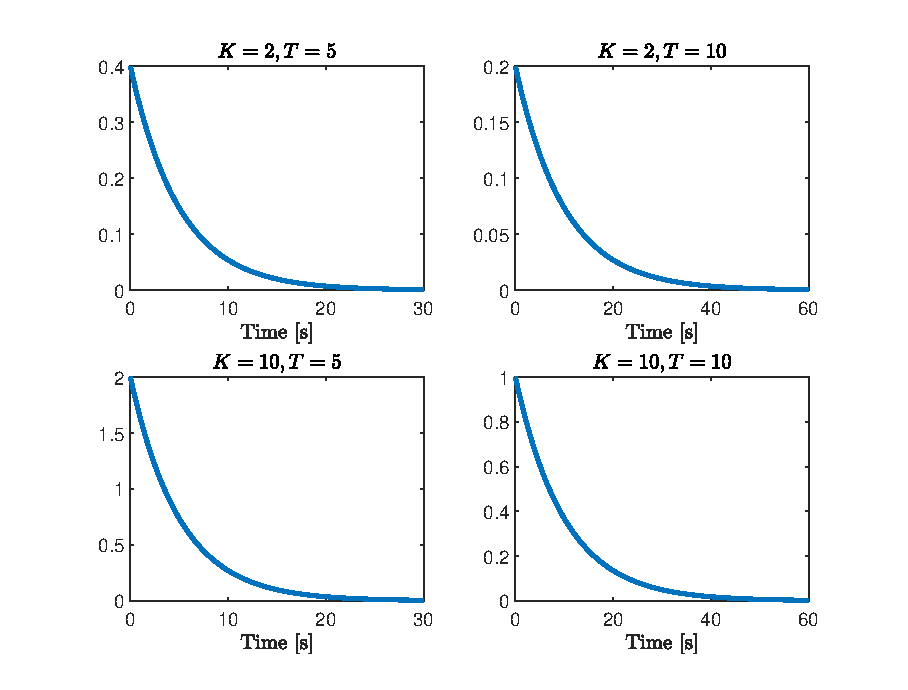
\includegraphics[width=.8\textwidth]{images/impulse_response.eps}
    \caption{Impulse response of 1\textsuperscript{st} order systems}
\end{figure}

%-------------------------------------------%
\subsubsection{Step Response of 1\textsuperscript{st} Order Systems}
%-------------------------------------------%
\[
U(s)=\frac{1}{s} 
\quad {\color{gray}\longrightarrow} \quad 
\boxed{G(s)=\frac{K}{Ts+1}} 
\quad {\color{gray}\longrightarrow} \quad  
Y(s)= \frac{1}{s}\frac{K}{Ts+1} 
\quad {\color{gray}\xrightarrow[]{\mathcal{L}^{-1}}} \quad  
y(t) = K(1-e^{-\frac{1}{T}t})
\]

\begin{figure}[H] 
    \centering 
    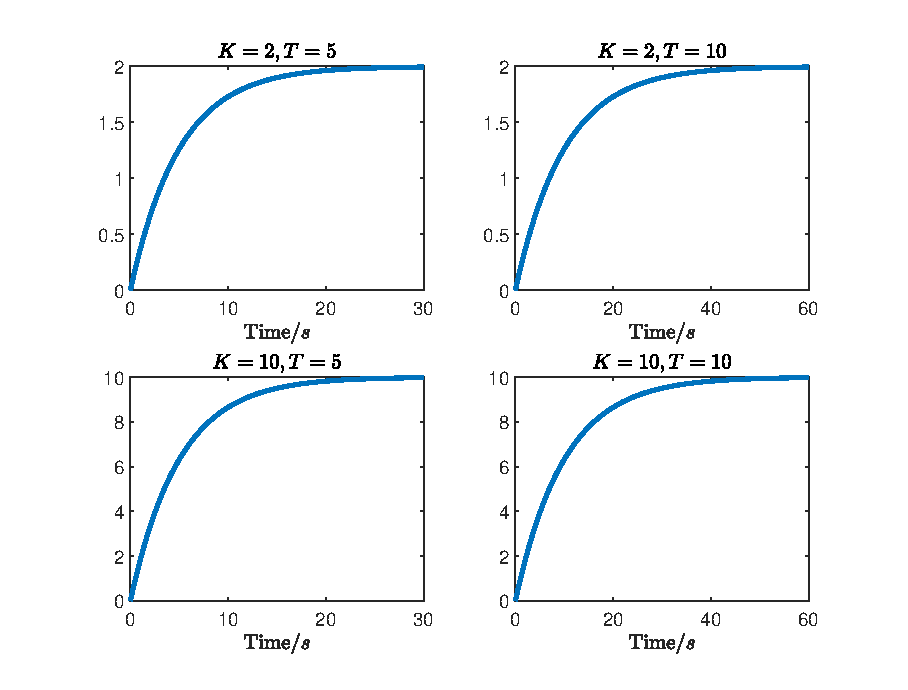
\includegraphics[width=.8\textwidth]{images/step_response.eps}
    \caption{Step response of 1\textsuperscript{st} order systems}
\end{figure}

%-------------------------------------------%
\subsection{Time Response Analysis for 2\textsuperscript{nd} Order Systems}
%-------------------------------------------%
\[\frac{\mathrm{d}^{2}y(t)}{\mathrm{d}t^{2}}+2\zeta\omega_{n}\frac{\mathrm{d}y(t)}{\mathrm{d}t}+\omega_{n}^{2}y(t) = K\omega_{n}^{2}u(t)\]
The transfer function for a $2^{nd}$ order system is $\displaystyle G(s)= \frac{K\omega_{n}^{2}}{s^{2}+2\zeta\omega_{n}s+\omega_{n}^{2}}$, where
\begin{itemize}
    \item $\zeta$ is \textbf{damping ratio}. It measures how much the system oscillates as the output decays towards the steady state.
    
    \item $\omega_{n}$ is \textbf{undamped natural frequency}. It measures how fast the system oscillates during the transient response.
\end{itemize}
Time response, $Y(s)$, of  $2^{nd}$ order systems:
\begin{itemize}
    \item Impulse response:\[Y(s)= \frac{K\omega_{n}^{2}}{s^{2}+2\zeta\omega_{n}s+\omega_{n}^{2}}\]
    
    \item Step response:\[Y(s)= \frac{K\omega_{n}^{2}}{s^{2}+2\zeta\omega_{n}s+\omega_{n}^{2}}\frac{1}{s}\]
\end{itemize}
The characteristic equations are both $s^{2}+2\zeta\omega_{n}s+\omega_{n}^{2}=0$, with poles at $s = (-\zeta\pm \sqrt{\zeta^{2}-1})\omega_{n}$.
This gives 3 cases: 
    \[
    s=\begin{cases}
    s = \pm j\omega_{n}\ ,&\zeta = 0\\
    s = (-\zeta\pm j\sqrt{1-\zeta^{2}})\omega_{n}\ , & 0<\zeta<1\\
    s = (-\zeta\pm \sqrt{\zeta^{2}-1})\omega_{n}\ , &\zeta>1\\
    \end{cases} 
    \]

%-------------------------------------------%
\subsubsection{\underline{Case 1:} $\zeta = 0$, Undamped Response}
%-------------------------------------------%
Undamped response happens when damping ratio $\zeta=0$, with poles at $s = \pm j\omega_{n}$.
The undamped step response is \textbf{purely sinusoidal}:
\[
Y(s) = \frac{K\omega_{n}^{2}}{s^{2}	+2\zeta\omega_{n}s+\omega_{n}^{2}}\frac{1}{s}
\quad  {\color{gray}\xrightarrow{\mathcal{L}^{-1}}} \quad
y(t) = K(1-\cos(\omega_{n}t)) 
\]

\begin{figure}[H] 
    \centering 
    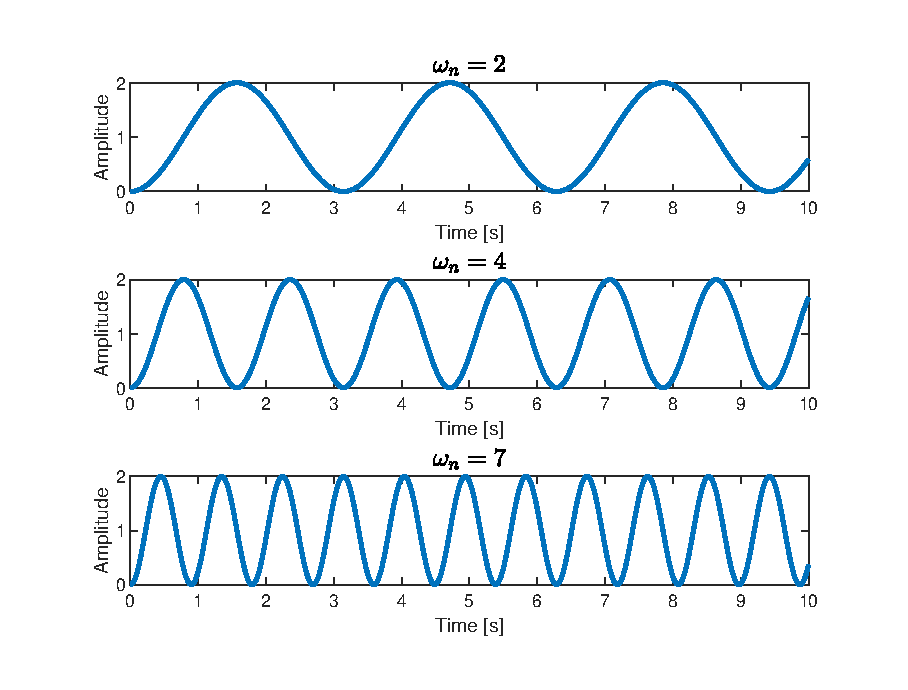
\includegraphics[width=.8\textwidth]{images/undamped_response.eps}
    \caption{Undamped response of 2\textsuperscript{nd} order systems. $K=1$}
\end{figure}

%-------------------------------------------%
\subsubsection{\underline{Case 2:} $0<\zeta<1$, Underdamped Response}
%-------------------------------------------%
Underdamped response happens when damping ratio $0<\zeta<1$, with 2 conjugate poles at $s = (-\zeta\pm j \sqrt{1-\zeta^{2}})\omega_{n}$.\\\\
The underdamped step response is \textbf{the combination of exponential function and sinusoidal function}:
\begin{itemize}
    \item Step response: 
    \[
    Y(s) = \frac{K\omega_{n}^{2}}{s^{2}	+2\zeta\omega_{n}s+\omega_{n}^{2}} \frac{1}{s} = K(\frac{1}{s}-\frac{s+\zeta\omega_{n}}{(s+\zeta\omega_{n})^{2}+\omega_{d}^{2}}-\frac{\zeta\omega_{n}}{(s+\zeta\omega_{n})^{2}+\omega_{d}^{2})})
    \]
    
    \item Take inverse Laplace transform:
    \[ {\color{gray}\xrightarrow{\mathcal{L}^{-1}}} \quad
    y(t) = K \bigg[ 1-\frac{e^{-\zeta\omega_{n} t}}{\sqrt{1-\zeta^{2}}} \sin(\omega_{d}t +\tan^{-1}\frac{\sqrt{1-\zeta^{2}}}{\zeta}) \bigg] 
    \]
    \begin{itemize}
        \item $\zeta\omega_{n}$ is known as \textbf{decay time constant};
        
        \item $\omega_{d}$ is known as \textbf{damped natural frequency} with the expression:
        \[\omega_{d} = \omega_{n}\sqrt{1-\zeta^{2}}\]
    \end{itemize}
\end{itemize}

\begin{figure}[H] 
    \centering 
    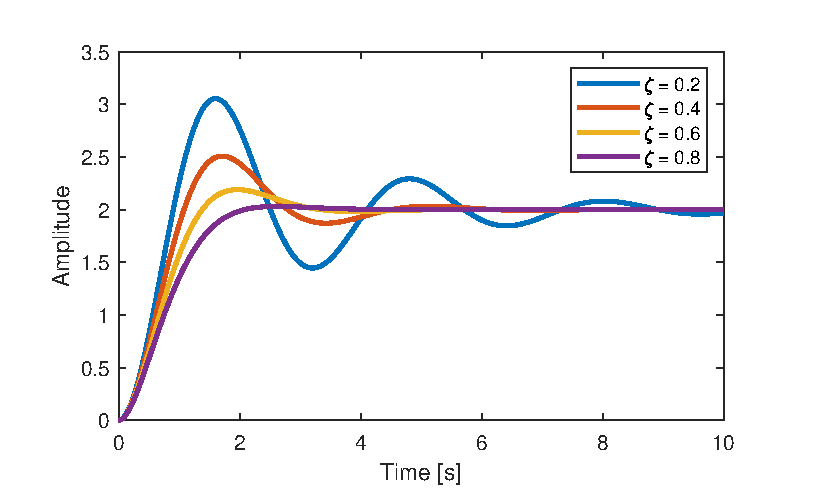
\includegraphics[width=.8\textwidth]{images/underdamped_response.eps}
    \caption{Underdamped response of 2\textsuperscript{nd} order systems. $\omega_{n}=2$, $K=2$}
\end{figure}

%-------------------------------------------%
\subsubsection{\underline{Case 3:} $\zeta>1$, Overdamped Response}
%-------------------------------------------%
Overdamped response happens when damping ratio $\zeta>1$, with 2 negative, real poles at $s = (-\zeta\pm \sqrt{\zeta^{2}-1})\omega_{n}$ which are refer as $\alpha$ and $\beta$.\\\\
The overdamped step response \textbf{quickly converges to a stable value}:
\begin{itemize}
    \item Step response:
    \[
    Y(s) = \frac{K\omega_{n}^{2}}{(s-\alpha)(s-\beta)} \frac{1}{s} = \frac{K\alpha\beta}{s(s-\alpha)(s-\beta)} = K\bigg[ \frac{1}{s}+\frac{1}{\alpha-\beta}(\frac{\beta}{s-\alpha}-\frac{\alpha}{s-\beta})\bigg]
    \]
    
\item Take inverse Laplace transform:
    \[
    {\color{gray}\xrightarrow{\mathcal{L}^{-1}}} \quad
    y(t) = K\bigg(1+\frac{\beta e^{\alpha t}-\alpha e^{\beta t}}{2\omega_{n}\sqrt{\zeta^{2}-1}}\bigg)
    \]
\end{itemize}

\begin{figure}[H] 
    \centering 
    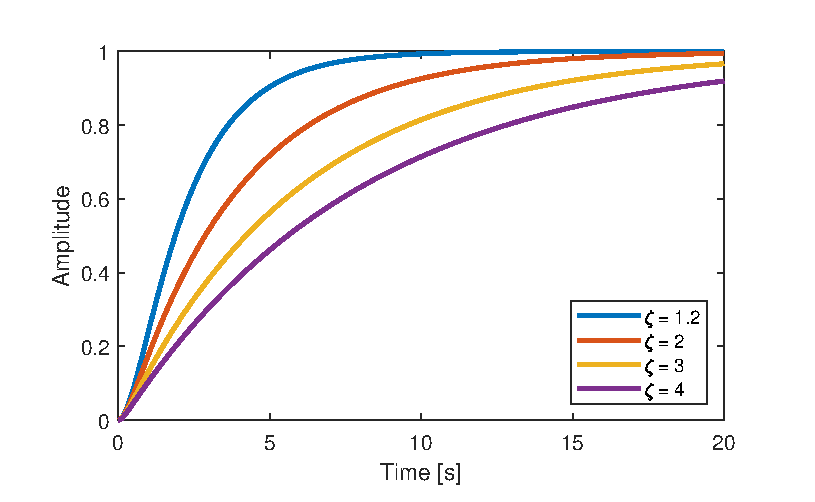
\includegraphics[width=.8\textwidth]{images/overdamped_response.eps}
    \caption{Overdamped response of 2\textsuperscript{nd} order systems. $\omega_{n}=1$, $K=1$}
\end{figure}

%-------------------------------------------%
\subsection{Transient Specification of 2\textsuperscript{nd} Order Systems}
%-------------------------------------------%
\begin{figure}[H] 
    \centering
    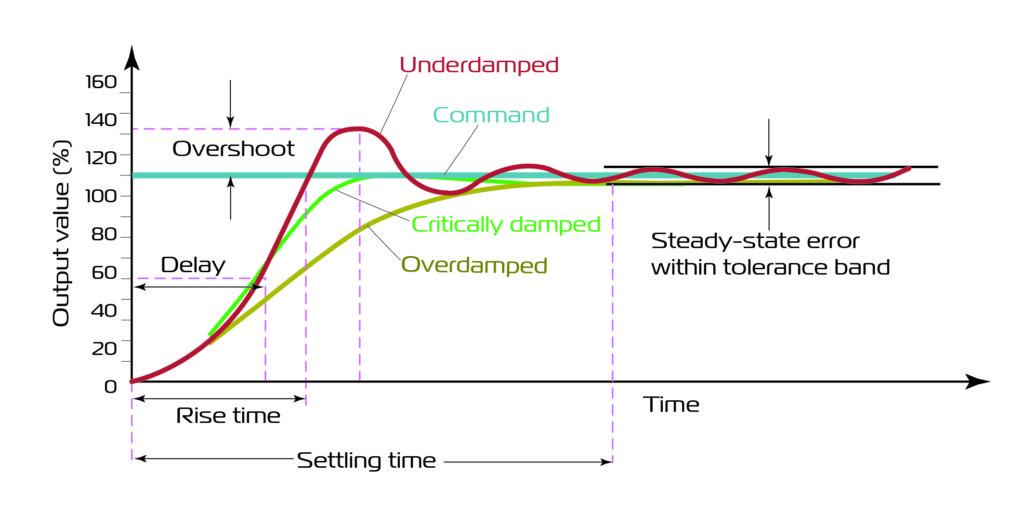
\includegraphics[width=0.8\textwidth]{images/PID_response.jpg}
    \caption{Overshoot, Rise time, Setting time and Steady-state error \protect\footnotemark}
\end{figure}
\footnotetext{Figure adopted from \href{https://www.motioncontroltips.com/how-to-address-overshoot-in-servo-control/}{https://www.motioncontroltips.com/how-to-address-overshoot-in-servo-control/}}

\begin{itemize}
    \item \textbf{Rise time, $t_{r}$:} the time taken for the output to go from 10\% to 90\% of the final value.
    \[t_{r} = \frac{\pi-\cos^{-1}\zeta}{\omega_{d}}\]
    
    \item \textbf{Peak time, $t_{p}$:} the time taken for the output to reach its maximum value.
    \[t_{p} = \frac{\pi}{\omega_{n}\sqrt{1-\zeta^{2}}}\]
    
    \item \textbf{2\% Settling time, $t_{s2\%}$:} the time taken for the signal to be bounded to within a tolerance of x\% (here, 2\%) of the steady state value.
    \[t_{s2\%} = \frac{4}{\zeta\omega_{n}}\]
    
    \item \textbf{Overshoot}: 
    \[\textbf{overshoot} = \frac{\text{max value - min value}}{\text{final value}}\times 100\]
    
    \item \textbf{Steady-state error}: the difference between the input step value and the final value.
\end{itemize}
